%%%%%%%%%%%%%%%%%%%%%%%%%%%%%%%%%%%%%%%%%
% a0poster Portrait Poster
% LaTeX Template
% Version 1.0 (22/06/13)
%
% The a0poster class was created by:
% Gerlinde Kettl and Matthias Weiser (tex@kettl.de)
% 
% This template has been downloaded from:
% http://www.LaTeXTemplates.com
%
% License:
% CC BY-NC-SA 3.0 (http://creativecommons.org/licenses/by-nc-sa/3.0/)
%
%%%%%%%%%%%%%%%%%%%%%%%%%%%%%%%%%%%%%%%%%

%----------------------------------------------------------------------------------------
%	PACKAGES AND OTHER DOCUMENT CONFIGURATIONS
%----------------------------------------------------------------------------------------

\documentclass[a0,portrait]{a0poster}

\usepackage{multicol} % This is so we can have multiple columns of text side-by-side
\columnsep=100pt % This is the amount of white space between the columns in the poster
\columnseprule=3pt % This is the thickness of the black line between the columns in the poster

\usepackage[svgnames]{xcolor} % Specify colors by their 'svgnames', for a full list of all colors available see here: http://www.latextemplates.com/svgnames-colors

\usepackage{times} % Use the times font
%\usepackage{palatino} % Uncomment to use the Palatino font

\usepackage{graphicx} % Required for including images
\usepackage{booktabs} % Top and bottom rules for table
\usepackage[font=small,labelfont=bf]{caption} % Required for specifying captions to tables and figures
\usepackage{amsfonts, amsmath, amsthm, amssymb} % For math fonts, symbols and environments
\usepackage{wrapfig} % Allows wrapping text around tables and figures
\usepackage{url}

\begin{document}

%----------------------------------------------------------------------------------------
%	POSTER HEADER 
%----------------------------------------------------------------------------------------

% The header is divided into two boxes:
% The first is 75% wide and houses the title, subtitle, names, university/organization and contact information
% The second is 25% wide and houses a logo for your university/organization or a photo of you
% The widths of these boxes can be easily edited to accommodate your content as you see fit

\begin{minipage}[b]{0.75\linewidth}
\veryHuge \color{NavyBlue} \textbf{RADISH: The System Balance of Power for Large Data Centers} \color{Black}\\ % Title
\Huge\textit{Evaluating Amdahl's Rules of Thumb with Google Cluster Data}\\[2cm] % Subtitle
\huge \textbf{Vincent Lee \& Shumo Chu}\\[0.5cm] % Author(s)
\huge University of Washington: Computer Science and Engineering\\[0.4cm] % University/organization
\end{minipage}
%
\begin{minipage}[b]{0.25\linewidth}

\includegraphics[width=20cm]{cse_logo.png}\\
\end{minipage}

\vspace{1cm} % A bit of extra whitespace between the header and poster content

%----------------------------------------------------------------------------------------

\begin{multicols}{2} % This is how many columns your poster will be broken into, a portrait poster is generally split into 2 columns

%----------------------------------------------------------------------------------------
%	ABSTRACT
%----------------------------------------------------------------------------------------

\color{Navy} % Navy color for the abstract

\section{Introduction}

The design of large data centers is driven by application workloads, performance targets, energy efficiency constraints, and system scalability.
To build these systems, we rely on empirical analysis and engineering intuition to properly allocate the amount of computation, memory, disk, and networking I/O to satisfy these contraints.
A system with insufficient resources will perform poorly as a single component of the system can bottleneck progress.
Alternatively, a system with over-provisioned resources is wasteful and can expend unnecessary energy and silicon area.
Ideally, we'd like to construct systems which have sufficient amounts of memory, compute, disk, and network I/O but at the same time not overprovision these resources.

%----------------------------------------------------------------------------------------
%	INTRODUCTION
%----------------------------------------------------------------------------------------

\color{SaddleBrown} % SaddleBrown color for the introduction

\section*{Amdahl's Rules of Thumb for a Balanced System}

\begin{center}\vspace{1cm}
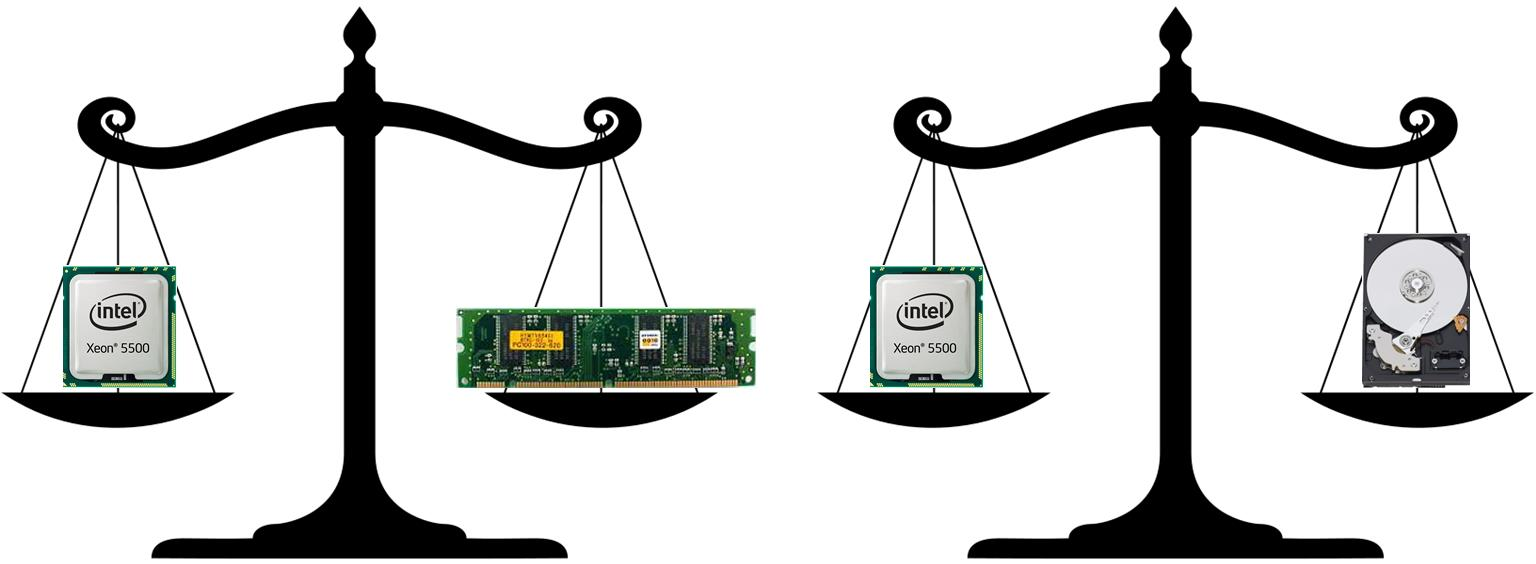
\includegraphics[width=0.8\linewidth]{balance_fig.jpg}
\end{center}\vspace{1cm}

\noindent Amdahl's Rules of Thumb for a balanced system proposed in suggest that an ideally balanced system roughly adhere to the following ratios: \\
\begin{enumerate}
\item \textbf{Amdahl's parallelism law}: if a computation has serial component S and parallel component P, then the maximum speedup is (S+P)/S \\
\item \textbf{Amdahl's balanced system law}: a system needs one bit of memory IO per second for each instruction per second \\
\item \textbf{Amdahl's memory law}: in a balanced system, the ratio $\alpha$ of the size of memory in MB to the instructions per second in million instructions per second (MIPS) is 1 MB per 1 MIPS or $\alpha = 1$ \\
\item \textbf{Amdahl's IO law}: programs do one memory IO per 50000 instructions
\end{enumerate}

%----------------------------------------------------------------------------------------
%	OBJECTIVES
%----------------------------------------------------------------------------------------

\color{DarkSlateGray} % DarkSlateGray color for the rest of the content

\section*{Main Objectives}

We seek to analyze the publically available Google Cluster Data trace.

The Google Cluster Data trace consists of job and task usage measurements recorded over a period of 29 days in May of 2009 at an undisclosed data center. 
Using the data trace, we seek to:

\begin{enumerate}
\item[1] Determine if it is possible to extract meaningful system balance ratios between compute, memory, disk, and networking I/O using the obfuscated traces, even order of magnitude calculations are sufficient.
\item[2] Determine what insights if any, these system balance ratios provide with respect to Amdahl's Rules of Thumb.
\end{enumerate}

We focus our attention on the task\_usage and task\_events traces which contain task granularity resource request quanities and actual usage records.

\begin{center}\vspace{1cm}
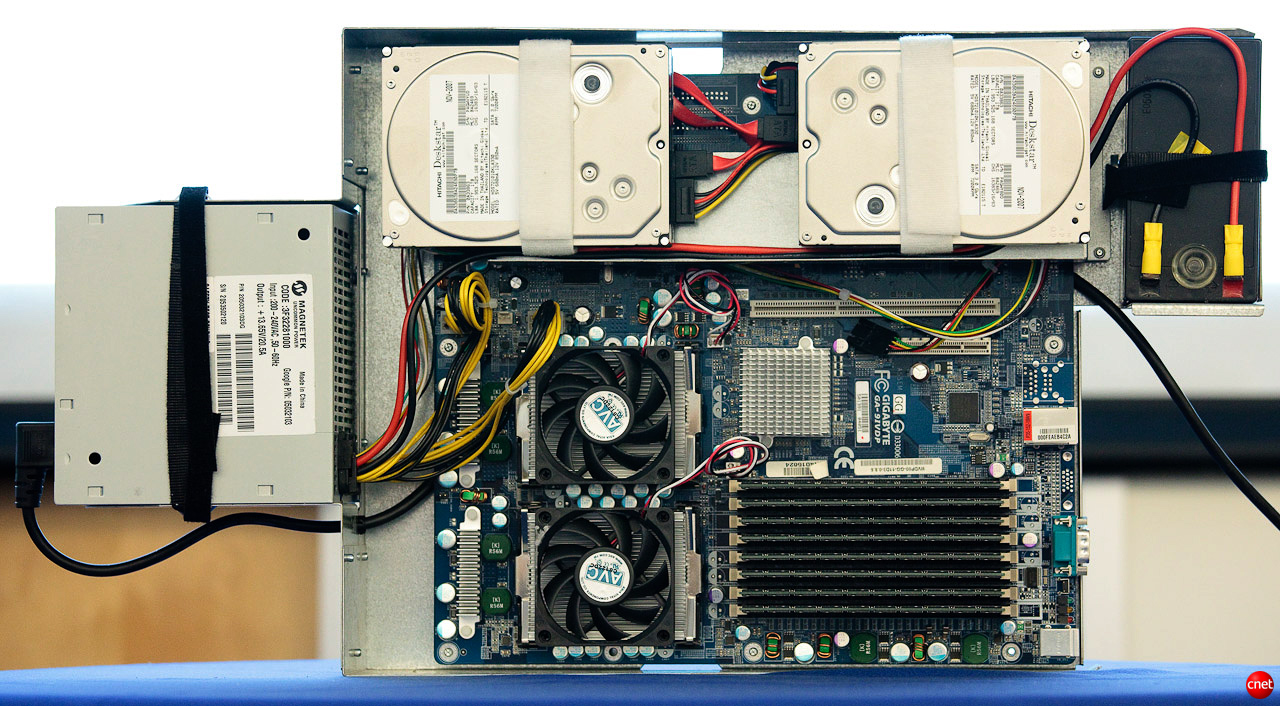
\includegraphics[width=0.8\linewidth]{GoogleServerLarge.jpg}
\captionof{figure}{\color{Green} Google server motherboard and components unveiled in 2009.}
\end{center}\vspace{1cm}

%----------------------------------------------------------------------------------------
%	RESULTS 
%----------------------------------------------------------------------------------------

\section*{Results}

\begin{center}\vspace{1cm}
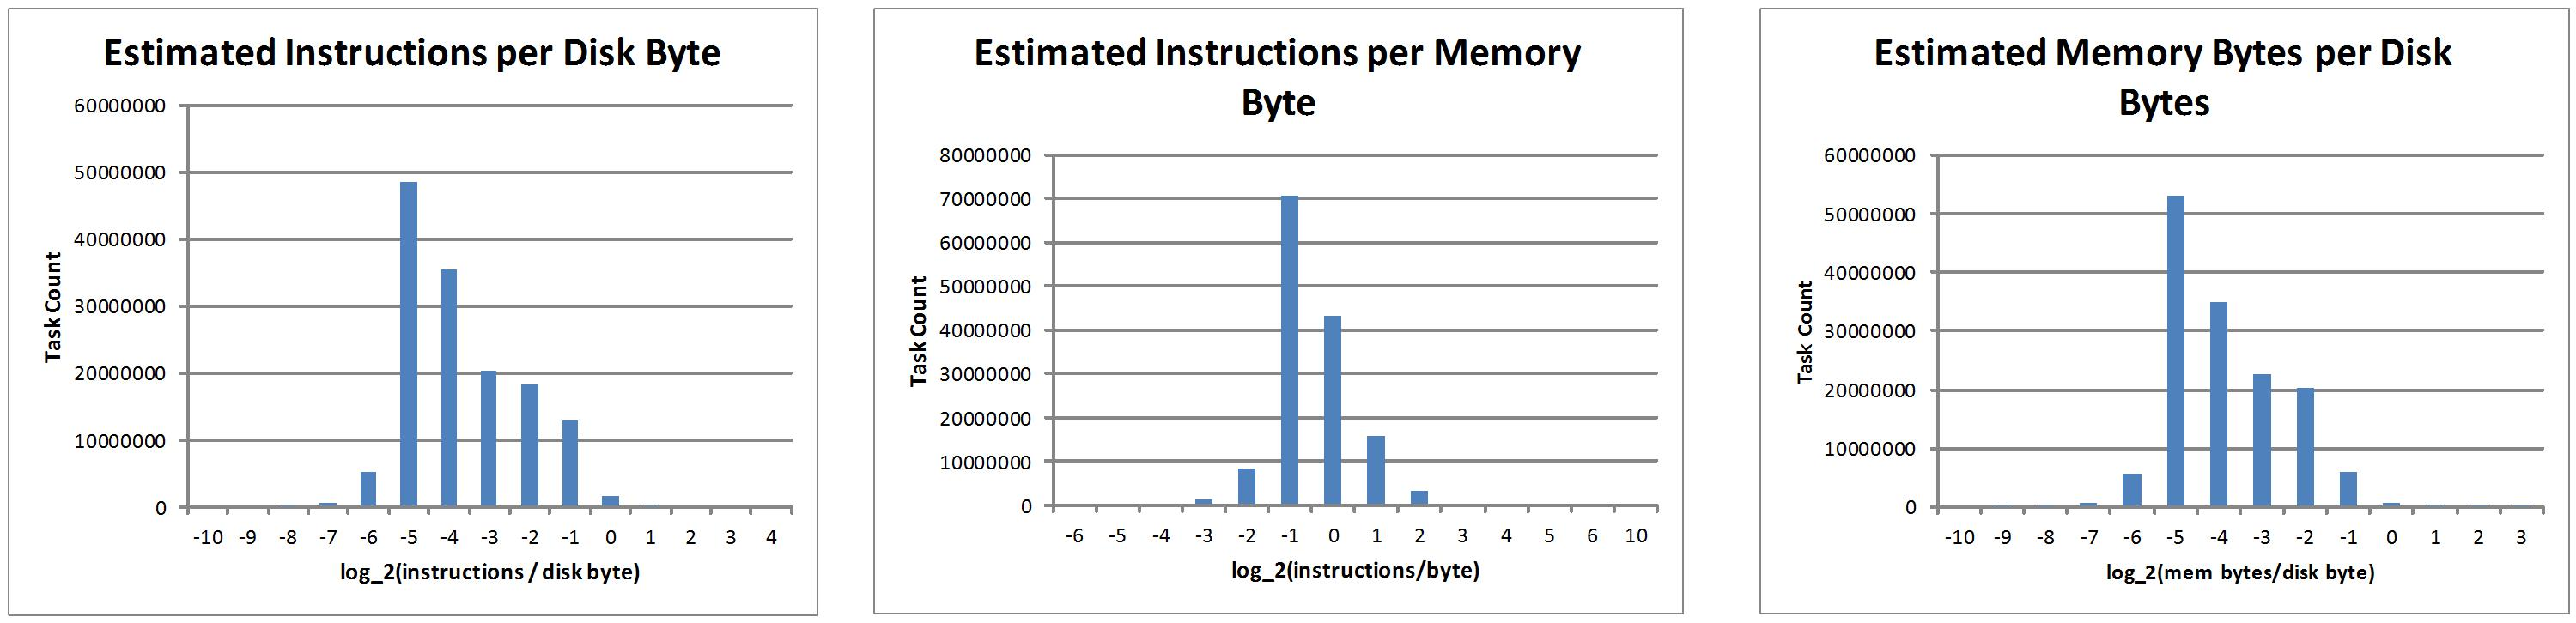
\includegraphics[width=0.9\linewidth]{request_distributions.jpg}
\captionof{figure}{\color{Green} Estimated system balance ratios for all task resource requests. Numbers are based on order of magnitude calculations for CPU count, CPU frequency, memory size, and disk space}
\end{center}\vspace{1cm}

\begin{center}\vspace{1cm}
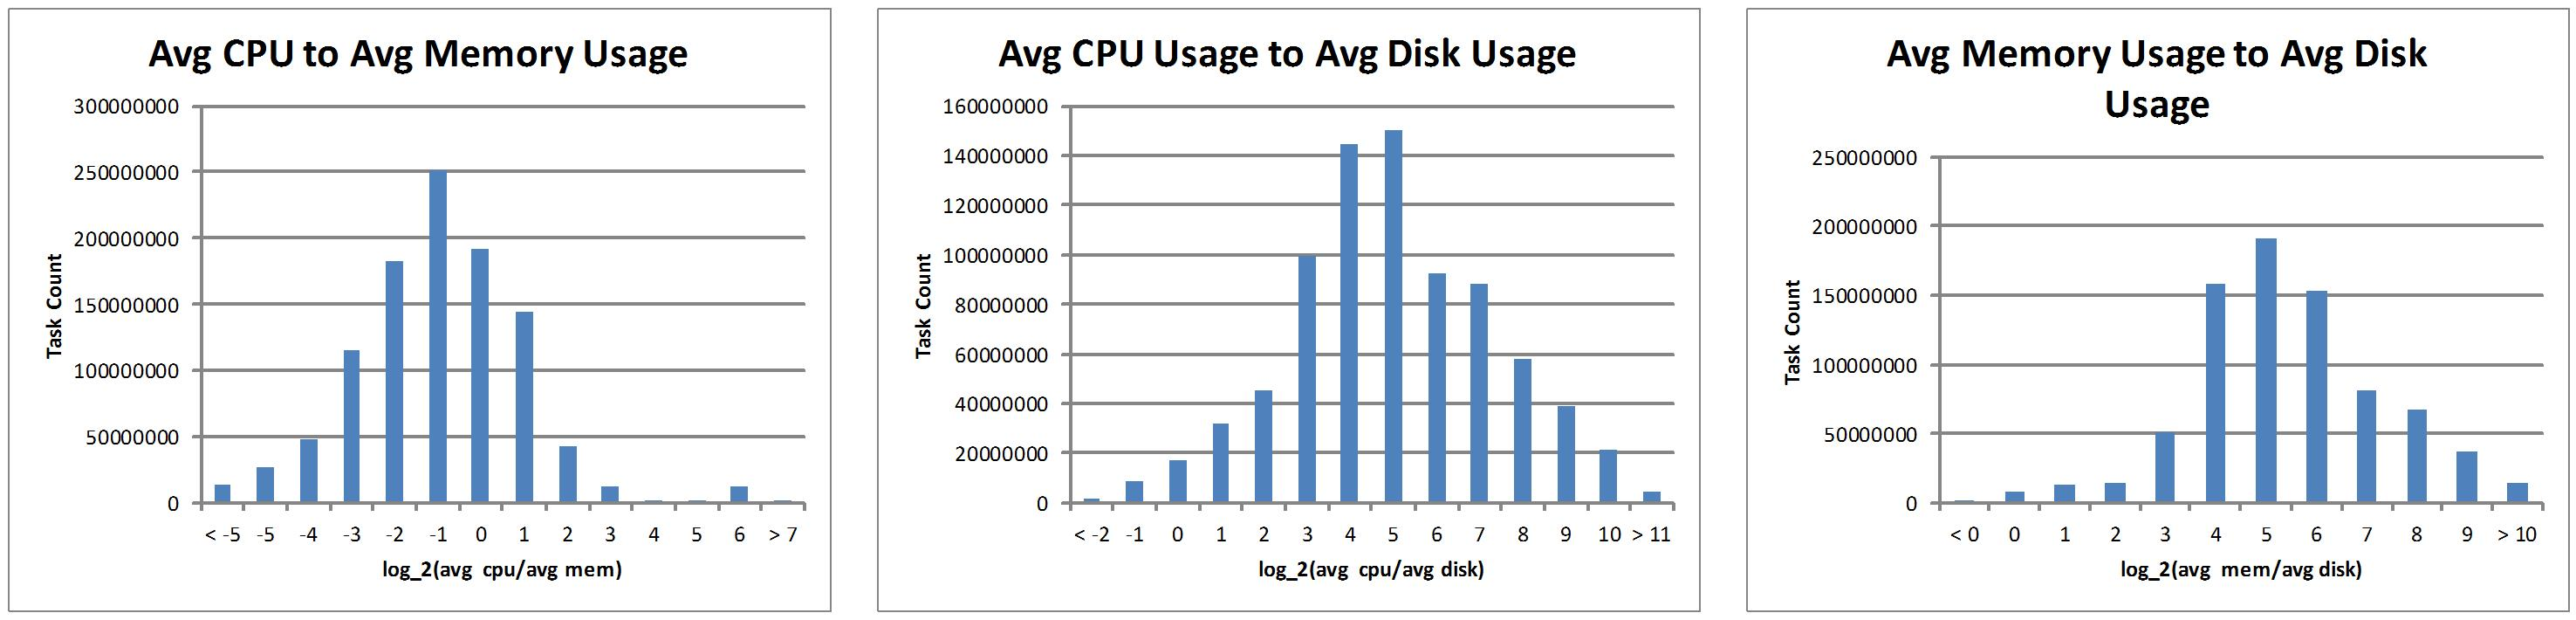
\includegraphics[width=0.9\linewidth]{actual_distributions.jpg}
\captionof{figure}{\color{Green} Relative system balance ratios for all task usage entries. Ratios represent relative usages using normalized values.}
\end{center}\vspace{1cm}


\begin{center}\vspace{1cm}
\begin{tabular}{| l | l l l l |} 
\toprule
\textbf{Quantity} & \textbf{Average} & \textbf{Est. Median} & \textbf{Min. Value} & \textbf{Max. Value} \\
\midrule
Req. CPU/Mem & 1.702 &  $2^{-1}$ & 0.00392 & 49160.986  \\ \hline
Est. Instr/Mem Byte & 1.702 & $2^{-1} $ & 0.00392 & 49160.986 \\ \hline
Req. CPU/Disk & 403.730 & $2^4$ & 203208.556 & 0.184 \\ \hline
Est. Instr/Disk Byte & 1.577 & $2^{-4}$ & 793.783 & 0.000719 \\ \hline
Req. Mem/Disk & 260.060 & $2^4$ & 130334.487 & 0.200 \\ \hline
Est. Mem Byte/Disk Byte & 1.0159&  $2^{-4}$ & 509.119 & 0.000781 \\ \hline
\bottomrule
\end{tabular}
\captionof{table}{Relative Task Usage Ratios - individual quantities are still normalized; estimated median is given in order of magnitude}
\end{center}\vspace{1cm}

\begin{center}\vspace{1cm}
\begin{tabular}{| l | l l l l |} 
\toprule
\textbf{Quantity} & \textbf{Average} & \textbf{Est. Median} & \textbf{Min. Value} & \textbf{Max. Value} \\
\midrule
Avg CPU/Avg Mem & 11.737 & $2^{-1}$ & 0.0000160 & 425920.100  \\ 
Avg CPU/Avg Disk & 2901.793 & $2^5$ & 0.000263 & 152878263.605 \\ 
Avg Mem/Avg Disk & 2253.51 & $2^5$ & 0.00102 & 579532.348 \\ 
Peak CPU/Peak Mem & 26.567 & & 0.0000194 & 2008293.839 \\ 
Avg CPU/(Avg Mem * CPI) & 9.949 & & 5.0193 & 293932.257 \\ 
Avg CPU/(Avg Disk * CPI) & 2443.536 & & 0.00000522 & 66671724.206 \\ 
\bottomrule
\end{tabular}
\captionof{table}{Relative Task Usage Ratios - individual quantities are still normalized}
\end{center}\vspace{1cm}

\begin{center}\vspace{1cm}
\begin{tabular}{| l | l l l |} 
\toprule
\textbf{Quantity} & \textbf{Average} & \textbf{Min. Value} & \textbf{Max. Value} \\
\midrule
Avg CPU Usage & 0.023 & 0 & 145.8 \\ \hline
Avg Memory Usage & 0.023 & 0 & 0.881 \\ \hline
Avg Local Disk Space & 0.000125 & 0 & 0.00726 \\ \hline
%Assigned Memory & 0.029 & 0.00000477 & 229100\* \\ \hline
Peak Memory Usage & 0.024 & 0 & 0.886 \\ \hline
Disk I/O Time & 0.00357 & 0 & 0.685 \\ \hline
Peak CPU Rate & 0.0904 & 0 & 1744\* \\ \hline
Peak Disk I/O Time & 0.0232 & 0 & 10.98 \\ \hline
CPI & 4.866 & 0 & 25370\* \\ \hline
MAI & 0.0176 & 0 & 8.5\* \\ \hline
\bottomrule
\end{tabular}
\captionof{table}{Task Usage Statistics - some maximum values are anamolous and can be attributed to bugs in the data collection infrastructure or task statistics aggregation}
\end{center}\vspace{1cm}


%----------------------------------------------------------------------------------------
%	CONCLUSIONS
%----------------------------------------------------------------------------------------

\color{SaddleBrown} % SaddleBrown color for the conclusions to make them stand out

\section*{Conclusions}

While we were not able to procure exact system balance ratios, our order of magnitude calculations still provide enough insight to re-evaluate Amdahl's Rules of Thumb: \\

\noindent \textbf{Amdahl's Parallelism Law} - clearly continues to hold \\
\textbf{Amdahl's Balanced System Law} - we are unable to comment on this rule as the trace does not contain bandwidth statistics\\
\textbf{Amdahl's Memory Law} - value for $\alpha$ indicating instruction per byte of memory is likely to be larger than 1, a trend predicted by J. Gray  and confirmed by our analysis\\
\textbf{Amdahl's IO law} - memory access per instruction is closer to one memory access per 50 or 500 instructions instead of one memory access per 50000 instructions \\

 %----------------------------------------------------------------------------------------
%	REFERENCES
%----------------------------------------------------------------------------------------

%\nocite{*} % Print all references regardless of whether they were cited in the poster or not
%\bibliographystyle{plain} % Plain referencing style
\bibliographystyle{abbrv}
\bibliography{poster.bib} % Use the example bibliography file sample.bib

\end{multicols}
\end{document}
